\chapter{Resultados adicionales}


\begin{table}[htbp]
\centering
\small
\caption{Taxonomía de SMOEAs. Adaptado de \cite{Shao2025_SMOEA}.}
\label{tab:taxonomia-smoea}
% Ajusta los anchos aquí: 3.5cm para la 1ra columna, 3.2cm para la 2da, 5.5cm para la 3ra
\begin{tabular}{|C{3.5cm}|C{3.2cm}|C{5.5cm}|}
\hline
\textbf{Categoría} & \textbf{Subcategoría} & \textbf{Métodos específicos} \\
\hline
\multirow{10}{3.5cm}{\centering 1. MOEAs basados en nuevos operadores de variación}
 & \multirow{5}{3.2cm}{\centering 1.1 Volteo de variables} & Volteo estático de variables \\
 & & Volteo dinámico de variables \\
 & & Volteo híbrido de variables \\
 & & Volteo adaptativo de variables \\
 & & Volteo robusto de variables \\
\cline{2-3}
 & \multirow{2}{3.2cm}{\centering 1.2 Optimización convexa} & Operador disperso convexo \\
 & & Operador de truncamiento disperso \\
\cline{2-3}
 & \multirow{3}{3.2cm}{\centering 1.3 Operador novedoso} & Muestreo de población dispersa \\
 & & Operador adaptativo \\
 & & Población múltiple \\
\hline
\multirow{5}{3.5cm}{\centering 2. MOEAs basados en reducción de dimensionalidad}
 & \multirow{3}{3.2cm}{\centering 2.1 Redes neuronales} & Red neuronal no supervisada \\
 & & Aprendizaje por refuerzo profundo \\
 & & Perceptrón multicapa \\
\cline{2-3}
 & 2.2 Minería de patrones & --- \\
\cline{2-3}
 & 2.3 Interacción biniveles & --- \\
\hline
\multirow{6}{3.5cm}{\centering 3. MOEAs basados en agrupación de variables de decisión}
 & \multirow{3}{3.2cm}{\centering 3.1 Agrupación uniforme} & Agrupación aleatoria \\
 & & Agrupación dinámica \\
 & & Agrupación de granularidad múltiple \\
\cline{2-3}
 & \multirow{3}{3.2cm}{\centering 3.2 Agrupación no uniforme} & Agrupación rápida \\
 & & Agrupación no uniforme \\
 & & Agrupación adaptativa \\
\hline
\end{tabular}
\end{table}


\begin{table}
\centering
\footnotesize
\caption{Fidelidad de la migración a C++ de los operadores genéticos respecto de su implementación original en PlatEMO/MATLAB.}
\label{tab:fidelidad_algoritmos}
\begin{tabular}{p{5cm}p{2cm}p{6cm}}
\hline
\textbf{Componente} & \textbf{Fidelidad} & \textbf{Notas} \\
\hline
\texttt{vssps} --- inicialización stripe & Alta & La lógica de franjas fue traducida fielmente respecto de la implementación original. \\
\texttt{ssbx} --- sparse SBX & Alta & Se implementó correctamente el manejo de posiciones \textit{zero/nonzero} y los intercambios aleatorios en casos de desajuste (\textit{mismatches}). \\
\texttt{spm} --- sparse PM & Alta & Se implementó correctamente la mutación tanto de los valores como del nivel de esparsidad. \\
\texttt{sm2target} & Alta & El comportamiento de este componente se mantuvo fiel al original. \\
\texttt{Environmental Selection \_NSGA2} & Alta & La traducción resultó fiel al original, incorporando además la corrección del error de conversión \textit{inf} $\rightarrow$ \textit{int}. \\
\hline
\end{tabular}
\end{table}

\begin{table}
\centering
\footnotesize
\caption{Funciones y utilidades de MATLAB, nativas o de \textit{toolbox}, sin equivalente directo en la biblioteca estándar de C++ o Eigen, junto con la estrategia de reimplementación adoptada y el tipo de equivalencia que dicha estrategia garantiza.}
\label{tab:funciones_sin_equivalente}
\begin{tabular}{p{2.9cm}p{2.6cm}p{3.5cm}p{4cm}}
\hline
\textbf{Función / utilidad MATLAB} & \textbf{Uso en el algoritmo} & \textbf{Estrategia en C++} & \textbf{Naturaleza de la equivalencia} \\
\hline
\texttt{kmeans(X,2)} (Statistics and Machine Learning Toolbox) & \texttt{SparsityAnalysis} de MOEA-CKF: separa las variables de decisión en significativas (SV) y no significativas (NSV) según su \textit{fitness} acumulado. & Algoritmo de Lloyd propio, restringido a $k=2$ sobre datos 1D (\texttt{kmeans2}), con partición por mediana como respaldo si algún clúster queda vacío. & Algorítmica: ambas minimizan la misma función objetivo (varianza intra-clúster), pero \texttt{kmeans} de MATLAB ejecuta por defecto múltiples reinicios con inicialización \textit{k-means++}, mientras la versión en C++ ejecuta una única pasada determinista. \\
\texttt{unique(A,'rows')} (núcleo de MATLAB) & \texttt{ENS\_SS}/\texttt{NDSort}, \texttt{TournamentSelection} y \texttt{Environmental Selection}: deduplica individuos u objetivos antes de ordenar o seleccionar. & \texttt{uniqueRows()}: tabla asociativa ordenada (\texttt{std::map}) para deduplicar más reconstrucción del vector de índices \texttt{loc}. & Exacta por construcción: misma definición de igualdad de fila y mismo orden lexicográfico de salida. \\
\texttt{hist(Loc,1:max(Loc))} (Statistics and Machine Learning Toolbox) & \texttt{ENS\_SS}: cuenta cuántas veces aparece cada fila única para saber cuántos individuos ya fueron ordenados. & Conteo directo por acumulación sobre el vector \texttt{loc} (\texttt{Table[l]++}), sin necesidad de definir \textit{bins}. & Exacta: mismo resultado, caso particular más simple al coincidir cada \textit{bin} con un índice de fila única. \\
\texttt{sortrows} / \texttt{sort(...,2)} (núcleo de MATLAB) & \texttt{TournamentSelection} (rango lexicográfico de \textit{fitness}) y truncamiento en \texttt{Environmental Selection} (orden de distancias). & \texttt{std::sort} con comparador lexicográfico sobre \texttt{std::vector<double>}. & Exacta: mismo orden total, mismo criterio de desempate. \\
\texttt{pdist2(A,B)} (Statistics and Machine Learning Toolbox) & Truncamiento por distancia: matriz de distancias euclidianas entre individuos del último frente. & Doble bucle explícito que evalúa la norma euclidiana fila a fila. & Exacta: misma fórmula cerrada $\|a-b\|_2$, sin aproximación. \\
\texttt{randi} / \texttt{randperm} / \texttt{unifrnd} (generador Mersenne Twister propio de MATLAB) & Inicialización de la población, mutación y selección estocásticas en ambos algoritmos. & Cabecera \texttt{<random>} de C++ & Ambos muestrean uniformemente de forma correcta, pero al tratarse de generadores pseudoaleatorios distintos las secuencias no coinciden aun fijando la misma semilla. \\
\hline
\end{tabular}
\end{table}

%-------------------------------------
\section{Resultados selección de framework de simulación}

\begin{table}[htbp]
\centering
\small
\caption{Tiempo de evaluación de \textit{fitness} en milisegundos con \(K = 30\). La columna \textit{Tendencia} indica si la correlación de Spearman entre iteración y tiempo fue significativa ($p<0.05$); el detalle se encuentra en la Sección~\ref{sec:anexo-independencia}.}
\label{tab:framework-evals-res}
\begin{tabular}{llrrrl}
\toprule
Config & Framework & \(n\) & Media \(\pm\) DE (ms) & Mediana (ms) & Tendencia \\
\midrule
ds1\_h10 & snn-simulator & 30 & 44.40 \(\pm\) 1.15   & 44.09 & sí \\
ds1\_h10 & ANNarchy      & 30 & 158.52 \(\pm\) 2.40  & 157.95 & no \\
ds1\_h10 & NEST          & 30 & 2475.41 \(\pm\) 1043.56 & 2418.16 & sí \\ \hline
ds1\_h20 & snn-simulator & 30 & 60.39 \(\pm\) 1.72   & 59.92 & sí \\
ds1\_h20 & ANNarchy      & 30 & 160.60 \(\pm\) 2.91  & 160.05 & no \\
ds1\_h20 & NEST          & 30 & 2601.42 \(\pm\) 1067.47 & 2547.92 & sí \\ \hline
ds4\_h10 & snn-simulator & 30 & 39.15 \(\pm\) 0.60   & 39.05 & no \\
ds4\_h10 & ANNarchy      & 30 & 77.62 \(\pm\) 0.53   & 77.52 & no \\
ds4\_h10 & NEST          & 30 & 1023.46 \(\pm\) 323.54 & 1019.55 & sí \\ \hline
ds4\_h20 & snn-simulator & 30 & 46.00 \(\pm\) 4.08   & 45.11 & no \\
ds4\_h20 & ANNarchy      & 30 & 77.95 \(\pm\) 1.67   & 77.52 & no \\
ds4\_h20 & NEST          & 30 & 1045.15 \(\pm\) 305.28 & 1046.18 & sí \\ \hline
ds3\_h10 & snn-simulator & 30 & 90.25 \(\pm\) 0.91   & 90.09 & no \\
ds3\_h10 & ANNarchy      & 30 & 254.58 \(\pm\) 2.97  & 255.19 & sí \\
ds3\_h10 & NEST          & 30 & 3841.14 \(\pm\) 1545.16 & 3922.09 & sí \\ \hline
ds3\_h20 & snn-simulator & 30 & 115.27 \(\pm\) 2.67  & 114.39 & no \\
ds3\_h20 & ANNarchy      & 30 & 257.45 \(\pm\) 3.37  & 257.13 & no \\
ds3\_h20 & NEST          & 30 & 3938.56 \(\pm\) 1489.22 & 4100.74 & sí \\
\bottomrule
\end{tabular}
\end{table}



\begin{table}[htbp]
\centering
\small
\caption{Tiempo de construcción y memoria pico por configuración y framework.}
\label{tab:framework-build-memory-res}
\begin{tabular}{llrr}
\toprule
Config & Framework & Construcción & Memoria pico \\
\midrule
ds1\_h10 & SNN-Simulator & 0.040 ms & 13.35 MB \\
ds1\_h10 & ANNarchy      & 773.39 ms (+ 9.79 s compilación Cython) & 4.63 MB \\
ds1\_h10 & NEST          & 3.04 ms  & 96.72 MB \\
ds1\_h20 & SNN-Simulator & 0.053 ms & 13.35 MB \\
ds1\_h20 & ANNarchy      & 762.32 ms (+ 9.69 s compilación) & 4.57 MB \\
ds1\_h20 & NEST          & 3.33 ms  & 97.11 MB \\
ds4\_h10 & SNN-Simulator & 0.072 ms & 13.35 MB \\
ds4\_h10 & ANNarchy      & 760.77 ms (+ 9.74 s compilación) & 4.71 MB \\
ds4\_h10 & NEST          & 5.21 ms  & 28.56 MB \\
ds4\_h20 & SNN-Simulator & 0.180 ms & 13.35 MB \\
ds4\_h20 & ANNarchy      & 768.38 ms (+ 9.69 s compilación) & 4.69 MB \\
ds4\_h20 & NEST          & 5.62 ms  & 29.01 MB \\
ds3\_h10 & SNN-Simulator & 0.037 ms & 13.35 MB \\
ds3\_h10 & ANNarchy      & 766.97 ms (+ 9.64 s compilación) & 4.59 MB \\
ds3\_h10 & NEST          & 3.51 ms  & 137.68 MB \\
ds3\_h20 & SNN-Simulator & 0.059 ms & 13.35 MB \\
ds3\_h20 & ANNarchy      & 764.19 ms (+ 9.82 s compilación) & 4.59 MB \\
ds3\_h20 & NEST          & 3.89 ms  & 138.08 MB \\
\bottomrule
\end{tabular}
\end{table}

%-------------------------------------
\section{Diagnóstico de independencia entre iteraciones en el \textit{benchmark} de \textit{frameworks}}
\label{sec:anexo-independencia}

Esta sección detalla los resultados del diagnóstico de independencia descrito en la Sección~\ref{sec:benchmark-framework-metodologia}. Para cada combinación de configuración y \textit{framework} se calculó la correlación de Spearman $\rho$ entre el número de iteración (0 a 29) y el tiempo de evaluación \texttt{eval\_s}, marcando como \textit{tendencia} los casos con $p<0.05$. Los resultados se presentan en la Tabla~\ref{tab:anexo-spearman}.

\begin{table}[htbp]
\centering
\small
\caption{Correlación de Spearman entre el número de iteración y el tiempo de evaluación ($n=30$ por celda). Se marca \textit{tendencia} cuando $p<0.05$. En las dos celdas de NEST con $\rho=1.000$ el valor $p$ calculado es numéricamente nulo.}
\label{tab:anexo-spearman}
\begin{tabular}{llrrl}
\toprule
Config & Framework & $\rho$ & $p$ & Tendencia \\
\midrule
ds1\_h10 & snn-simulator & $-0.515$ & $3.6\times10^{-3}$  & sí \\
ds1\_h10 & ANNarchy      & $-0.156$ & $0.409$             & no \\
ds1\_h10 & NEST          & $0.9996$ & $2.9\times10^{-44}$ & sí \\ \hline
ds1\_h20 & snn-simulator & $-0.399$ & $0.029$             & sí \\
ds1\_h20 & ANNarchy      & $-0.031$ & $0.869$             & no \\
ds1\_h20 & NEST          & $0.9991$ & $4.8\times10^{-40}$ & sí \\ \hline
ds4\_h10 & snn-simulator & $0.093$  & $0.624$             & no \\
ds4\_h10 & ANNarchy      & $-0.121$ & $0.525$             & no \\
ds4\_h10 & NEST          & $0.9987$ & $1.4\times10^{-37}$ & sí \\ \hline
ds4\_h20 & snn-simulator & $0.061$  & $0.750$             & no \\
ds4\_h20 & ANNarchy      & $0.117$  & $0.537$             & no \\
ds4\_h20 & NEST          & $0.9991$ & $4.8\times10^{-40}$ & sí \\ \hline
ds3\_h10 & snn-simulator & $-0.253$ & $0.177$             & no \\
ds3\_h10 & ANNarchy      & $-0.372$ & $0.043$             & sí \\
ds3\_h10 & NEST          & $1.000$  & $\approx 0$         & sí \\ \hline
ds3\_h20 & snn-simulator & $-0.294$ & $0.115$             & no \\
ds3\_h20 & ANNarchy      & $-0.070$ & $0.715$             & no \\
ds3\_h20 & NEST          & $1.000$  & $\approx 0$         & sí \\
\bottomrule
\end{tabular}
\end{table}

La tendencia de NEST es de signo positivo y de magnitud casi perfecta en las seis configuraciones, mientras que las tendencias detectadas en el simulador propio (\texttt{ds1\_h10} y \texttt{ds1\_h20}) y en ANNarchy (\texttt{ds3\_h10}) son de signo negativo y moderadas ($|\rho|\leq 0.52$). La Tabla~\ref{tab:anexo-nest-crecimiento} cuantifica el crecimiento de NEST: entre la primera y la última iteración de una misma corrida, el tiempo de evaluación se multiplica entre 2.8 y 5.5 veces. En las seis configuraciones el mínimo de NEST coincide con su primera iteración, es decir, el momento en que aún no se ha acumulado estado, y aun así es entre 12 y 17 veces mayor que el mínimo del simulador propio.

\begin{table}[htbp]
\centering
\small
\caption{Crecimiento del tiempo de evaluación de NEST dentro de una corrida y comparación del mínimo de NEST con el del \textit{snn-simulator}.}
\label{tab:anexo-nest-crecimiento}
\begin{tabular}{lrrrr}
\toprule
Config & Iteración 0 (ms) & Iteración 29 (ms) & Factor de crecimiento & Mín.\ NEST / mín.\ \textit{snn-simulator} \\
\midrule
ds1\_h10 &  752.6 & 4106.7 & 5.46 & 17.1 \\
ds1\_h20 &  859.9 & 4210.5 & 4.90 & 14.4 \\
ds4\_h10 &  502.9 & 1547.3 & 3.08 & 12.9 \\
ds4\_h20 &  540.9 & 1511.5 & 2.79 & 12.0 \\
ds3\_h10 & 1345.5 & 6620.7 & 4.92 & 15.0 \\
ds3\_h20 & 1485.2 & 6523.8 & 4.39 & 13.0 \\
\bottomrule
\end{tabular}
\end{table}

Como evidencia complementaria sobre el origen de la tendencia, se comparó la memoria pico de NEST entre dos corridas del mismo \textit{benchmark} que diferían únicamente en el número de repeticiones $K$. En una corrida previa, las configuraciones \texttt{ds3} se habían ejecutado con $K=15$ para acotar el tiempo total de medición, y posteriormente se aumentaron a $K=30$ para igualar el tamaño de muestra entre todas las configuraciones. Los valores de $K=15$ provienen del registro de esa corrida previa. En las configuraciones \texttt{ds1} y \texttt{ds4}, donde $K$ no cambió, la memoria de NEST se mantuvo idéntica entre ambas corridas. La Tabla~\ref{tab:anexo-nest-memoria} resume la comparación para \texttt{ds3}.

\begin{table}[htbp]
\centering
\small
\caption{Memoria pico de NEST en las configuraciones \texttt{ds3} al duplicar el número de repeticiones $K$.}
\label{tab:anexo-nest-memoria}
\begin{tabular}{lrrr}
\toprule
Config & Memoria con $K=15$ (MB) & Memoria con $K=30$ (MB) & Factor \\
\midrule
ds3\_h10 & 66.55 & 137.68 & 2.07 \\
ds3\_h20 & 66.94 & 138.08 & 2.06 \\
\bottomrule
\end{tabular}
\end{table}

La memoria de NEST creció de forma aproximadamente proporcional a $K$, mientras que la del \textit{snn-simulator} se mantuvo constante (13.35 MB, Tabla~\ref{tab:framework-build-memory-res}). Este patrón sugiere que NEST acumula estado entre evaluaciones sucesivas dentro de un mismo proceso, lo que es coherente con el aumento monótono del tiempo observado en la Tabla~\ref{tab:anexo-spearman}.

\paragraph{Alcance y limitaciones.} La correlación de Spearman detecta tendencias monótonas, pero no otras formas de dependencia serial (por ejemplo, autocorrelación sin tendencia), por lo que el diagnóstico se interpreta como un aviso de validez y no como una prueba formal de independencia. Del mismo modo, el crecimiento de la memoria es una evidencia indirecta: respalda la existencia de acumulación de estado, pero no se identificó qué componente de NEST la produce ni se probó que sea la causa única del aumento del tiempo. En conjunto, los resultados son consistentes con una violación del supuesto de independencia entre iteraciones en NEST. Dado que el tiempo crece a lo largo de la corrida, los tiempos de NEST reportados son, si acaso, una subestimación de su costo en corridas largas, sin alterar la conclusión del \textit{benchmark}. Aislar el efecto, por ejemplo mediante un proceso nuevo de NEST por iteración, queda como trabajo futuro.

%-------------------------------------
\section{Conectividad de las redes --- Dataset 4 (Sonar)}
\label{sec:anexo-conectividad-ds4}

Las Figuras~\ref{fig:anexo-conectividad-ds4-ckf} y~\ref{fig:anexo-conectividad-ds4-nsga} muestran, para MOEA-CKF y S-NSGA-II respectivamente, la solución de mejor exactitud de una corrida representativa de \texttt{ds4} (Sonar), seleccionada con el mismo criterio y bajo la misma convención de colores que la Figura~\ref{fig:conectividad-ejemplo} del Capítulo~\ref{chapter:resultados} (verde: viva; roja: muerta; naranjo: sumidero; amarillo: fuente; estrellas rojas: neuronas de salida). Se presentan por separado y a mayor tamaño, en vez de como subfiguras agrupadas, debido a que \texttt{ds4} tiene 60 características de entrada —más del doble que cualquier otro dataset del estudio (Tabla~\ref{tab:datasets_resumen})—, lo que hace ilegible una versión reducida con las 60 etiquetas de entrada.

\begin{figure}[htbp]
\centering
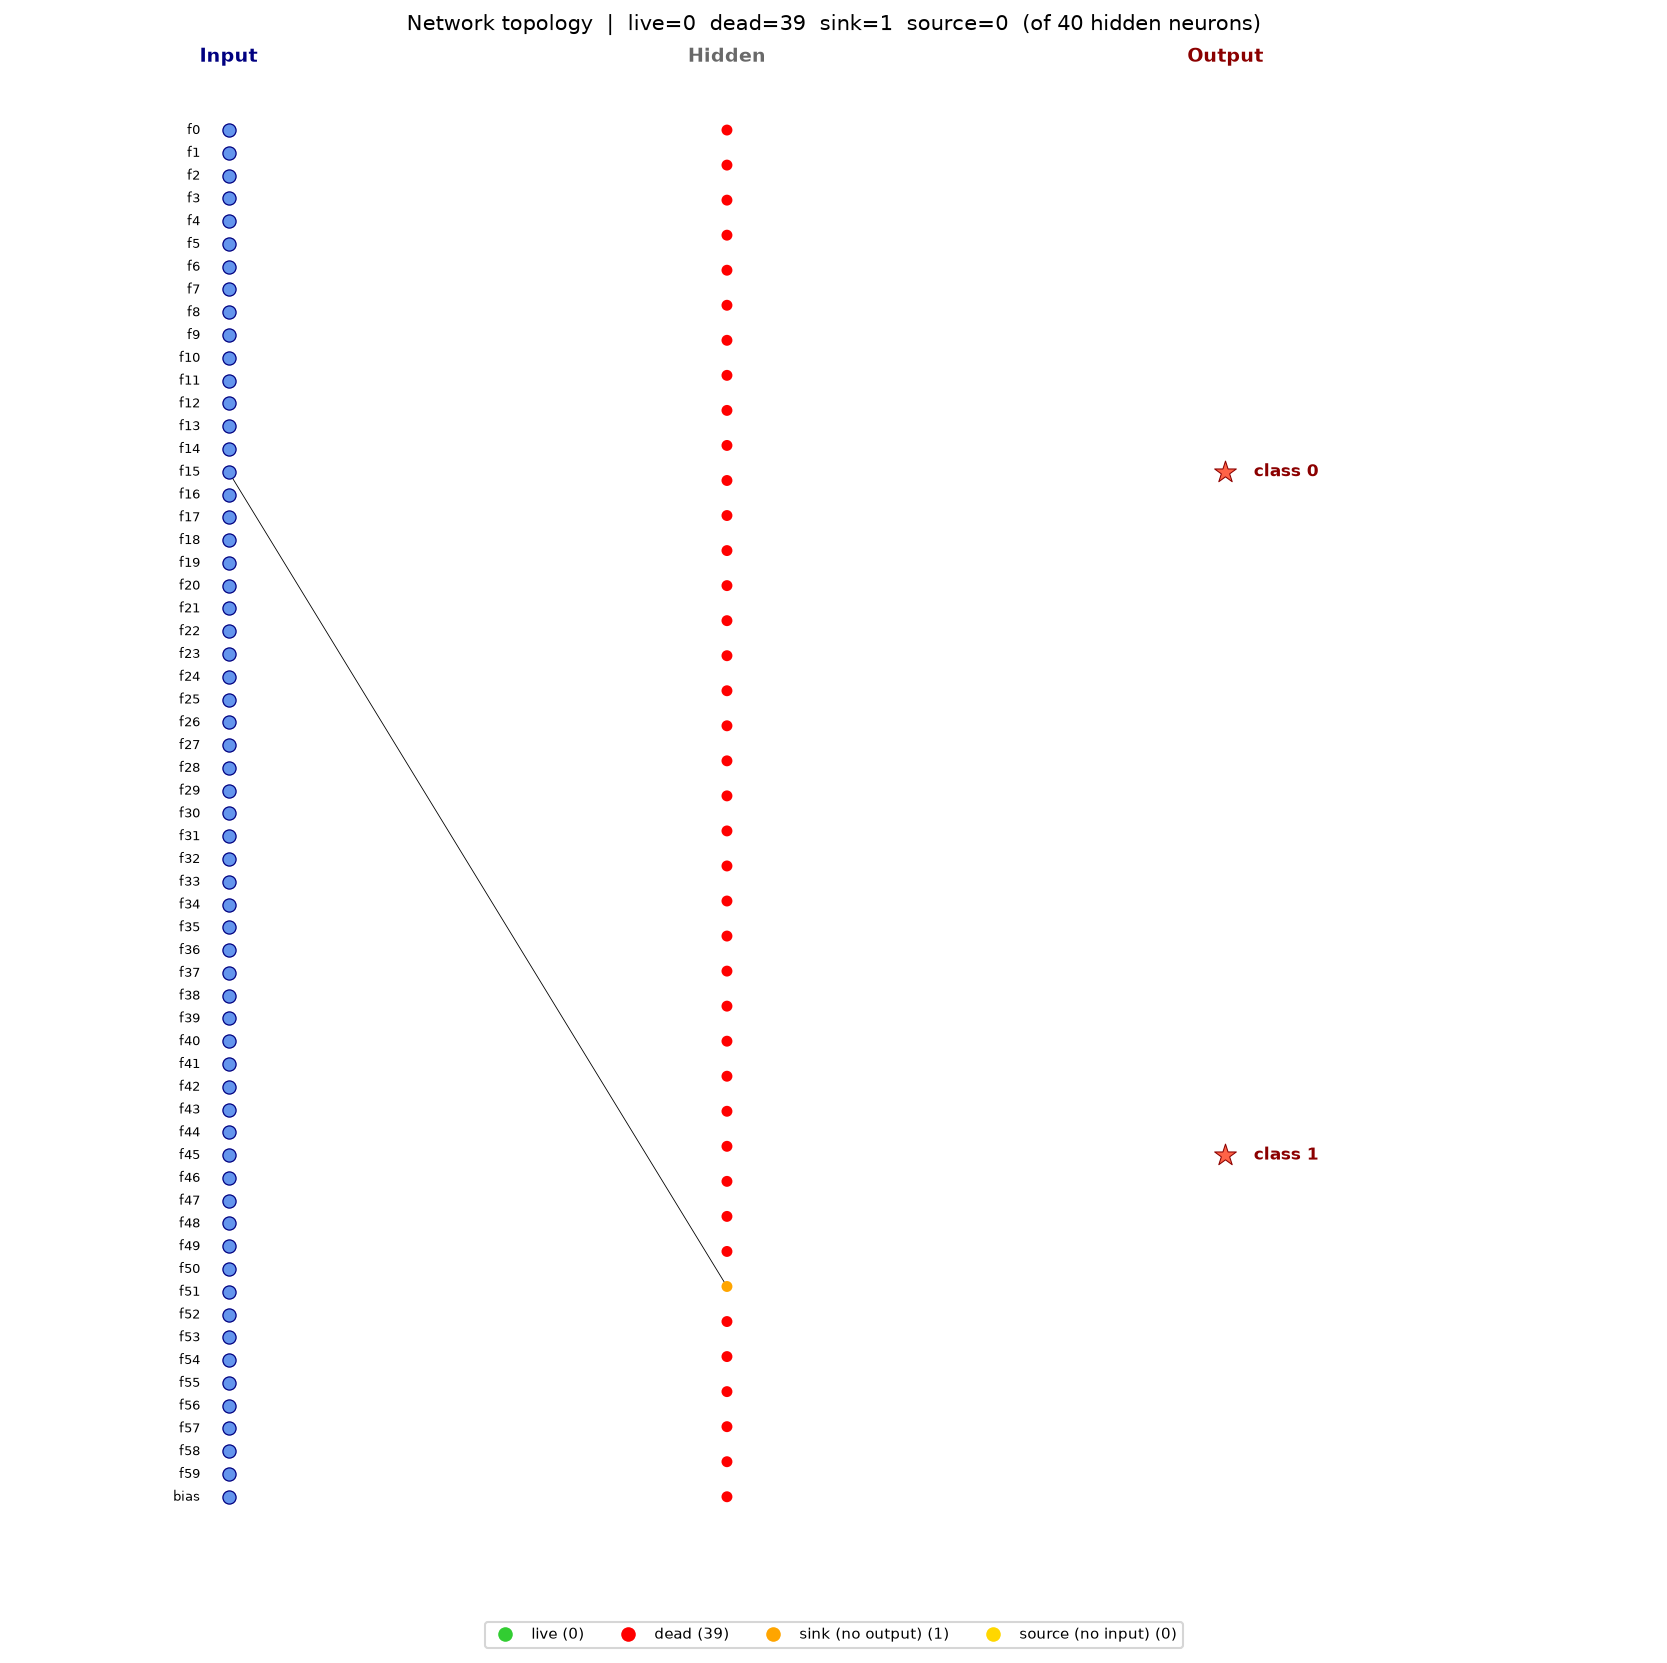
\includegraphics[width=0.85\textwidth]{images/conectividad_ds4_moeackf.png}
\caption{ds4-MOEA-CKF (corrida 14). Fila 7 de la Tabla~\ref{tab:conectividad-combo}: ilustra el problema de conexiones inútiles (100\% en esta corrida, 63.9\% en promedio) junto con clase de salida desconectada.}
\label{fig:anexo-conectividad-ds4-ckf}
\end{figure}

\begin{figure}[htbp]
\centering
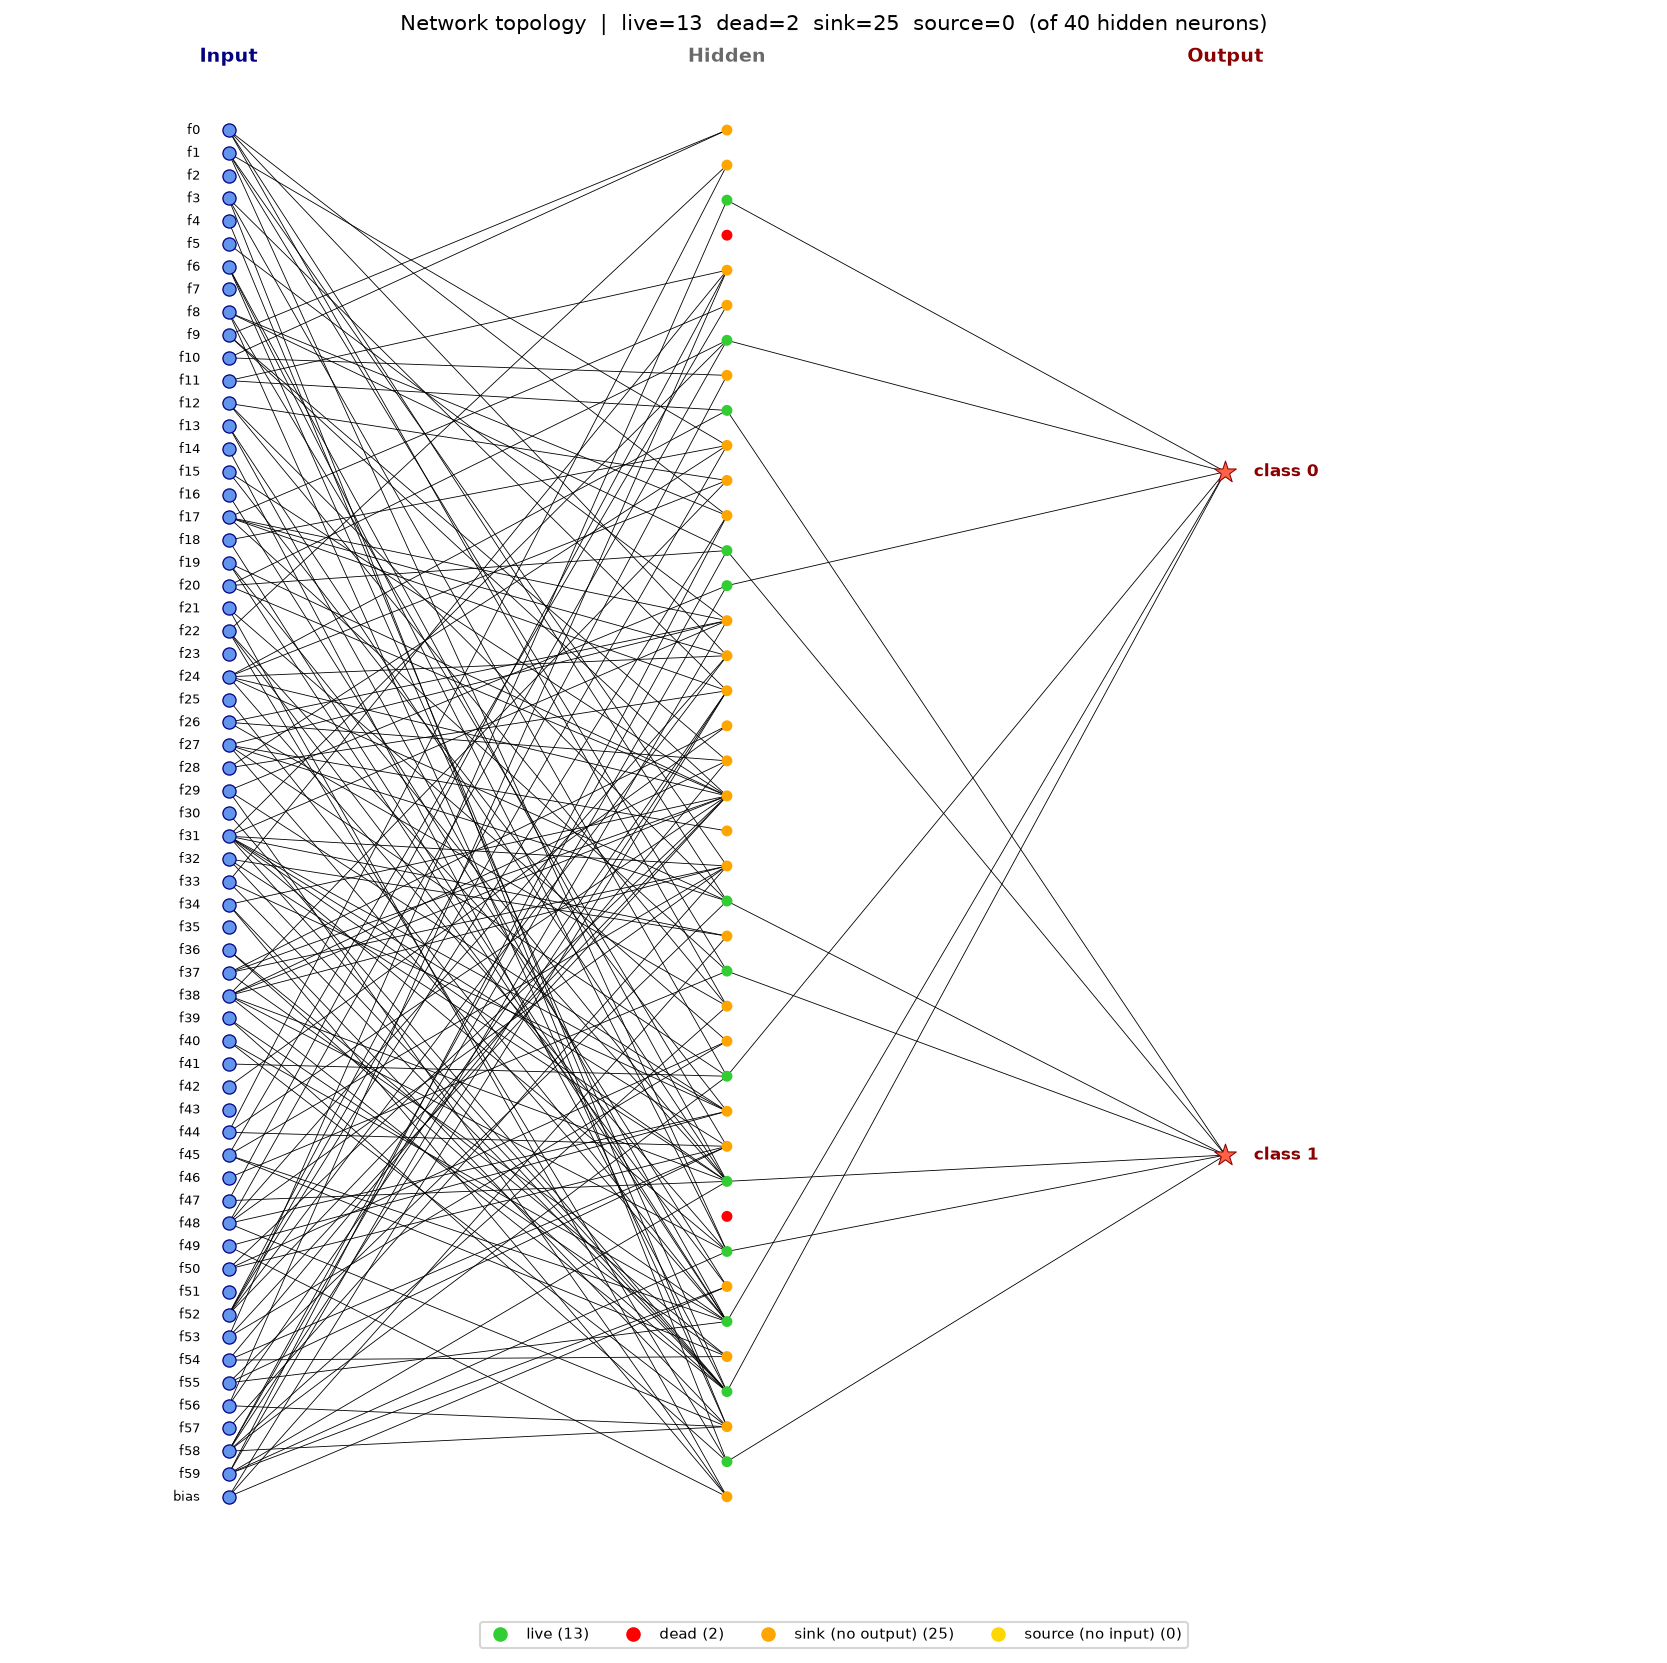
\includegraphics[width=0.85\textwidth]{images/conectividad_ds4_snsgaii.png}
\caption{ds4-S-NSGA-II (corrida 2). Fila 8 de la Tabla~\ref{tab:conectividad-combo}: ilustra principalmente el problema de conexiones inútiles (60.1\% en esta corrida, 57.0\% en promedio), sin clases de salida desconectadas.}
\label{fig:anexo-conectividad-ds4-nsga}
\end{figure}
